\DiaryEntry{Overlapping Events}{2021-12-21}{Stochastic}

\subsection{Event Start in the Unit Interval}

This is based on the entry\ref{2016-08-24:entry} and extends it.

\todo{Insert link to mathpages}

We have two events $A$ and $B$, starting randomly in the interval $[0,1]$ with start times $t_{A,1}$ and $t_{B,1}$, respectively. Each event has a deterministic duration; event $A$ has duration $w_A$, event $B$ has duration $w_B$. The end times of the events are denoted as $t_{A,2}$ and $t_{B,2}$, respectively and we have

\bee
t_{i,2} = t_{i,1} + w_i, \quad i \in \{A, B\}
\eee

Note that therefore, the end time of the events may be outside the unit interval.

The condition that the two events are overlapping is given by

\bee
(t_{B,1} < t_{A,1} < t_{B_2}) \vee (t_{A,1} < t_{B,1} < t_{A,2})
\eee

Assume that we have a realisation of $t_{A,1}$; for an overlap to happen, the corresponding realisation of $t_{B,1}$ must be in the interval $[t_{A,1}, t_{A,2}$. This is shown in the following Figure.

\begin{figure}[H]
    \centering
    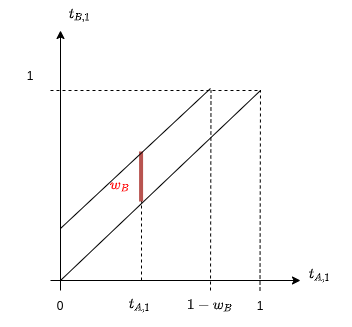
\includegraphics[scale=0.75]{images/2021-12-21_conc_events_1.png}
\end{figure}

This reasoning holds for all values of $t_{A,1}$ inside the unit interval. For $t_{A,1} > 1-w_B$, the possible values of $t_{B,1}$ are smaller, as $t_{B,1}$ is constrained to the unit interval as well. We can make the same arguments for a realisation of $t_{B,1}$. The complete picture is shown in the Figure below.

\begin{figure}[H]
    \centering
    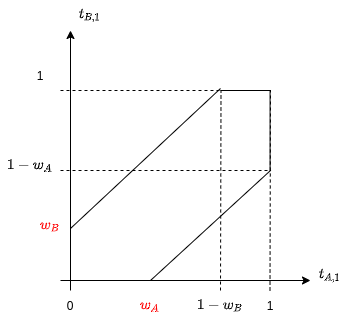
\includegraphics[scale=0.75]{images/2021-12-21_conc_events_2.png}
\end{figure}

The probability for an overlap equals the area inside the solid lines. It is given by

\bee
P = 1 - \frac{1}{2}(1 - w_A)^2 - \frac{1}{2}(1 - w_B)^2 = w_A + w_B - \frac{1}{2} w_A^2 - \frac{1}{2} w_B^2
\eee

For the special case of $w_A = 1$, the probability becomes

\bee
P = 1 + w_B - \frac{1}{1} - \frac{1}{2} w_B^2 = \frac{1}{2} + w_B(1 - \frac{1}{2}w_B)
\eee

This may seem counter-intuitive at first (if one event has a duration of one, we would expect the probability of an overlap to be one), but note that the event $A$ could start at $1$ (only the start time is in the unit interval). We will consider the case that the events are constrained inside the unit interval in the next Subsection.

If both interval lengths are equal to one, we obtain

\bee
P = 1 + 1 - \frac{1}{2} - \frac{1}{2} = 1
\eee

which matches the intuition.


\subsection{Event in the Unit Interval}

Now we consider the slightly different case where the \emph{whole event} is located inside the unit interval. Using the same naming conventions as above, this means that

\bee
t_{i,1} \sim \Uc(0, 1 - w_i), \quad i \in \{A,B\}
\eee

and implies $t_{i,2} < 1$.

Fix again the value of $t_{A,1}$. For an overlap to happen, the realisation of $t_{B,1}$ must be in the interval $[t_{A,1}, t_{A,2}]$; note however, that $t_{B,2} < 1$.

Finding a closed-form expression seems to be difficult (as we have two different uniform distributions); however, we see that the probability for an overlap is higher in this case than in the previous one. In addition, $P = 1$ for $w_A + w_B \geq 1$ as in this case the intervals will overlap for sure.

%%% Local Variables:
%%% mode: latex
%%% TeX-master: "journal"
%%% End:
